%%
%% Copyright (c) 2018 Weitian LI <liweitianux@sjtu.edu.cn>
%% Creative Commons BY 4.0
%%

% Class options:
%   bachelor|master|doctor	% 必选项
%   fontset=fandol|adobe|windows
%   oneside|twoside
%   openany|openright
%   zihao=-4|5			% 正文字号: 小四、五号(默认)
%   english			% 启用英文模版
%   review			% 盲审论文,隐去作者姓名、学号、
%				% 导师姓名、致谢、发表论文和参与的项目
%   submit			% 定稿提交的论文,插入签名扫描版的
%				% 原创性声明、授权声明
\documentclass[doctor, openright, twoside]{sjtuthesis}


\defaultfontfeatures{Mapping=tex-text}
\setmainfont{TeX Gyre Pagella}
\setsansfont{TeX Gyre Heros}
\setmonofont{M+ 1mn}
\setmathfont{TeX Gyre Pagella Math}

\setCJKmainfont[ItalicFont={Noto Sans CJK SC}]{Noto Serif CJK SC}
\setCJKsansfont{AR PL KaitiM GB}
\setCJKmonofont{Noto Sans Mono CJK SC}
\xeCJKsetup{PunctStyle=kaiming}


\title{射电晕对探测宇宙再电离信号的影响}
\keywords{%
\newcommand{\email}[1]{\href{mailto:#1}{\texttt{#1}}}
  低频射电天文,
  宇宙再电离时期,
  射电晕,
  弱信号分离,
  深度学习,
  卷积自编码器%
}
\author{李维天}
\studentnumber{0130729026}
\advisor{徐海光~教授}
\school{上海交通大学}
\institute{物理与天文学院}
\major{物理学}
\defenddate{2018 年 mm 月 dd 日}

\englishtitle{\textsc{%
  The Impacts of Radio Halos on Detecting the
  Epoch of Reionization Signal
}}
\englishkeywords{%
  low-frequency radio astronomy,
  epoch of reionization,
  radio halos,
  weak signal separation,
  deep learning,
  convolutional autoencoder%
}
\englishauthor{\textsc{Weitian Li}}
\englishadvisor{Prof. \textsc{Haiguang Xu}}
\englishinstitute{School of Physics and Astronomy}
\englishschool{Shanghai Jiao Tong University}
\englishlocation{Shanghai, China}
\englishmajor{Physics}
\englishdate{mmm dd, 2018}


\addbibresource{references.bib}


\begin{document}

\maketitle

\makeatletter
\ifsjtu@submit\relax
  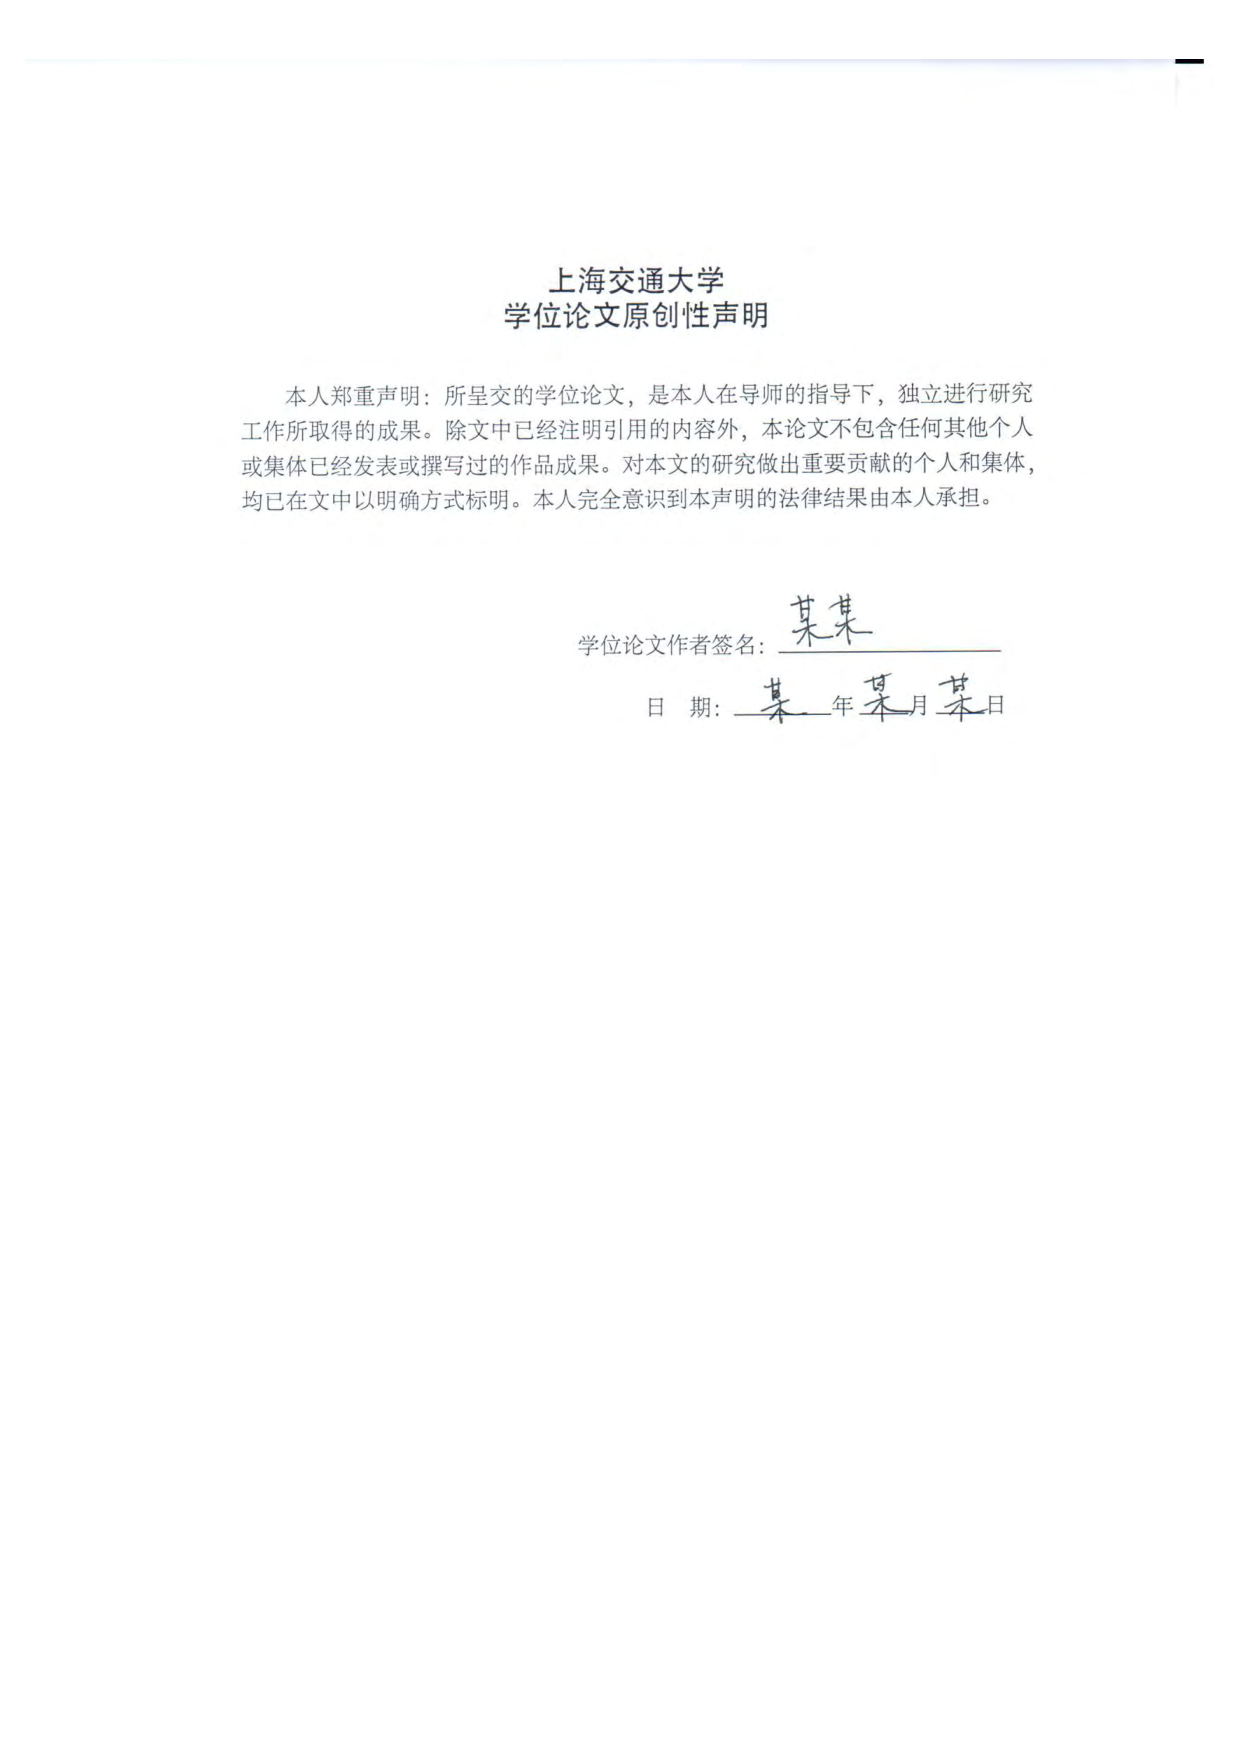
\includepdf{pdf/originality.pdf}
  \pdfbookmark[0]{\sjtu@label@originality}{originality}
  \cleardoublepage
  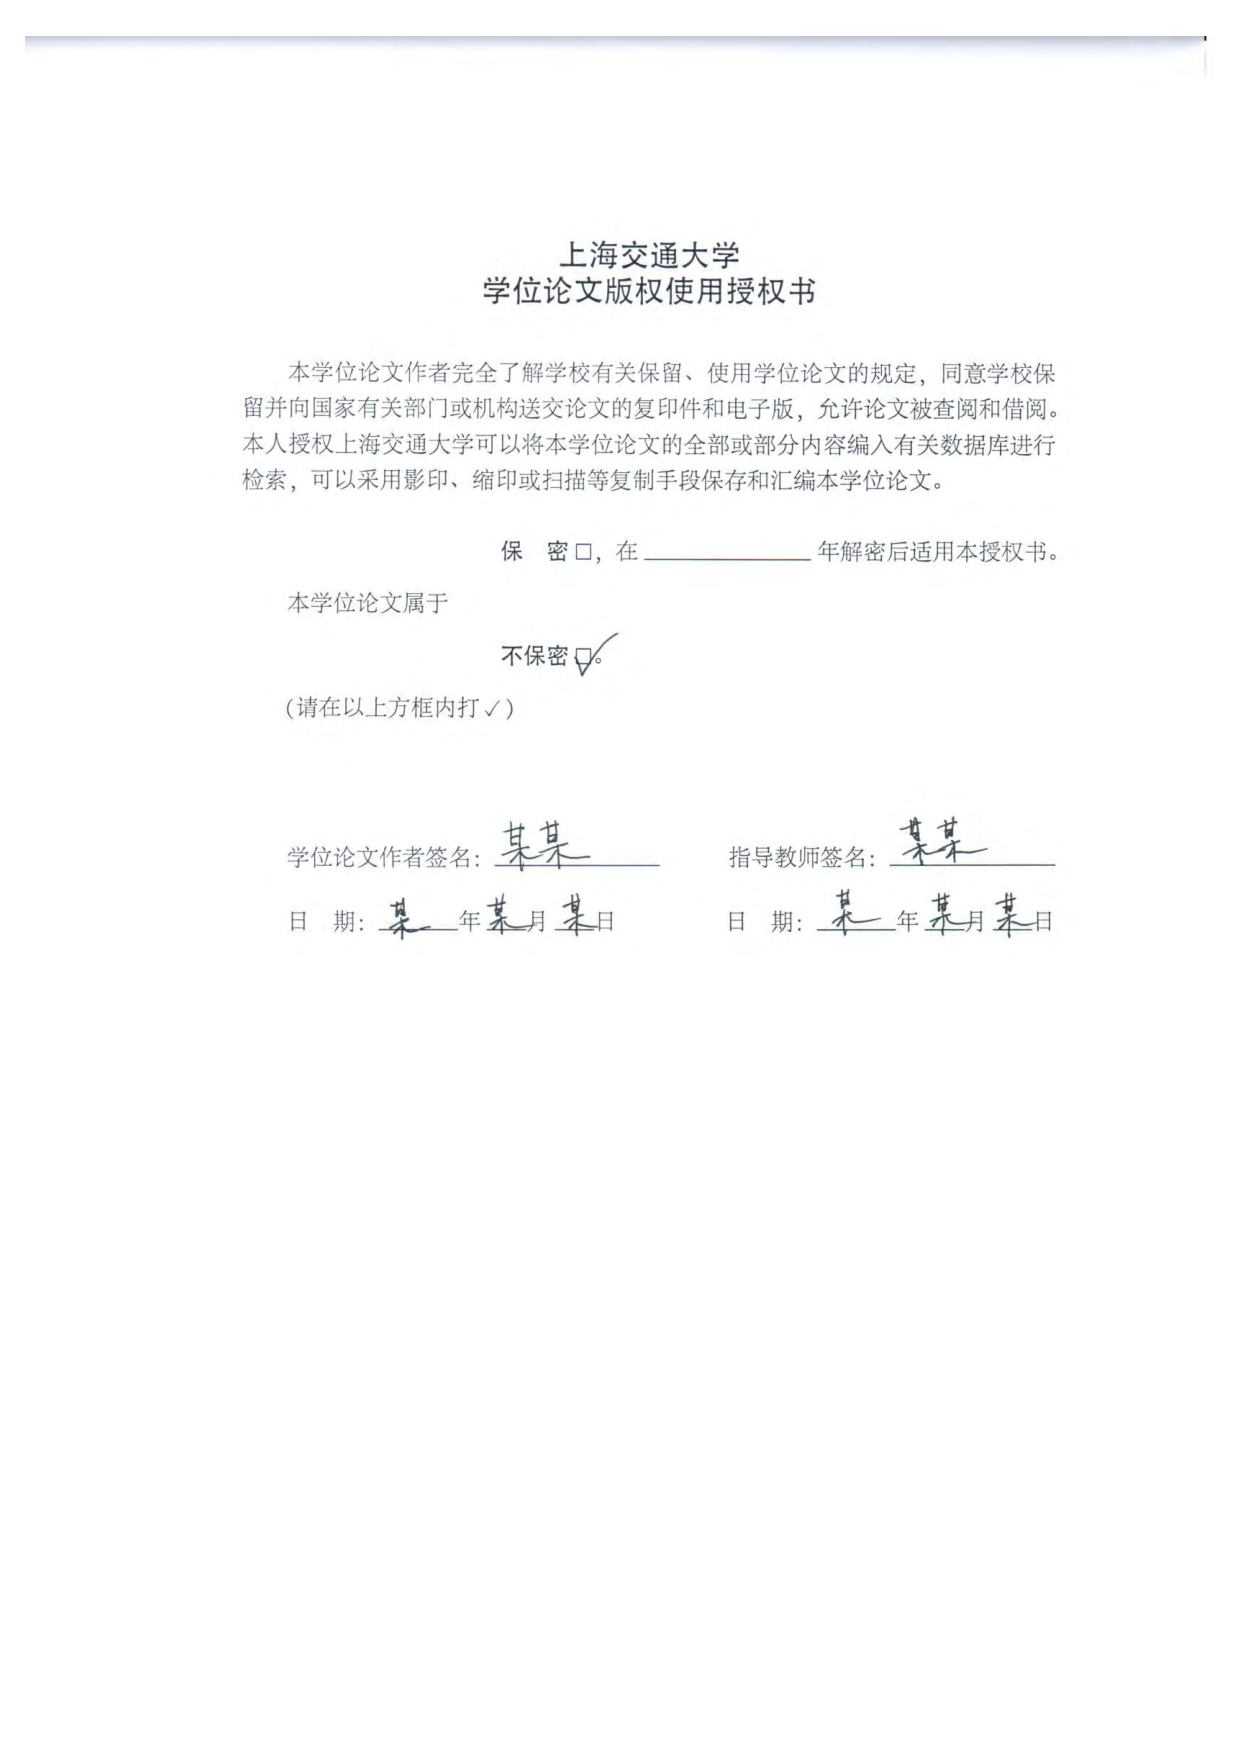
\includepdf{pdf/authorization.pdf}
  \pdfbookmark[0]{\sjtu@label@authorization}{authorization}
  \cleardoublepage
\else
\ifsjtu@review\relax
% exclude the originality and authorization declarations
\else
  \makeDeclareOriginality
  \makeDeclareAuthorization
\fi
\fi
\makeatother

\frontmatter

%%
%% Copyright (c) 2018 Weitian LI <liweitianux@sjtu.edu.cn>
%% Creative Commons BY 4.0
%%

% 中文摘要,约 3000 字
\begin{abstract}
\acl*{rh}如何影响 EoR 探测...
\end{abstract}

%---------------------------------------------------------------------

\begin{englishabstract}
\acs*{rh} can impose serious contamination on the EoR detection ...
\end{englishabstract}


\tableofcontents
\listoffigures
\addcontentsline{toc}{chapter}{\listfigurename}
\listoftables
\addcontentsline{toc}{chapter}{\listtablename}
% \listofalgorithms
% \addcontentsline{toc}{chapter}{\listalgorithmname}

\begin{nomenclaturename}
\label{chap:symb}

\begin{longtable}{rl}
$\epsilon$     & 介电常数 \\
 $\mu$ 		& 磁导率 \\
 $\epsilon$     & 介电常数 \\
 $\mu$ 		& 磁导率 \\
\end{longtable}

\end{nomenclaturename}


\mainmatter
\pagestyle{main}

%%
%% Copyright (c) 2018-2019 Weitian LI <liweitianux@sjtu.edu.cn>
%% Creative Commons BY 4.0
%%

\chapter{绪论}
\label{chap:introduction}

%=====================================================================
\section{研究背景}
\label{sec:background}

理解宇宙的结构、起源和演化,是人类孜孜不倦地追求的目标,在哲学和科学中占据重要地位.
经过无数人的努力,宇宙学的\ac{bbt}终于得以建立.
该理论已被大量观测证据所支持,比如星系的红移--距离关系(即 Hubble 定律)、
\ac{cmb}辐射、星系的大尺度分布、早期元素丰度、等等,
是目前宇宙学的标准模型.

根据大爆炸宇宙学模型,宇宙起源于约 138 亿年前的一次大爆炸,然后随着宇宙的膨胀,
温度以及能量密度都逐渐降低,宇宙主要经历了\ac{inflation}、\ac{bbn}、
\ac{recomb}、\ac{da}、形成第一代天体、\ac{reion}、形成星系及大尺度结构
等阶段,如\autoref{fig:univ-history} 所示.

\begin{figure}[!htp]
  \centering
  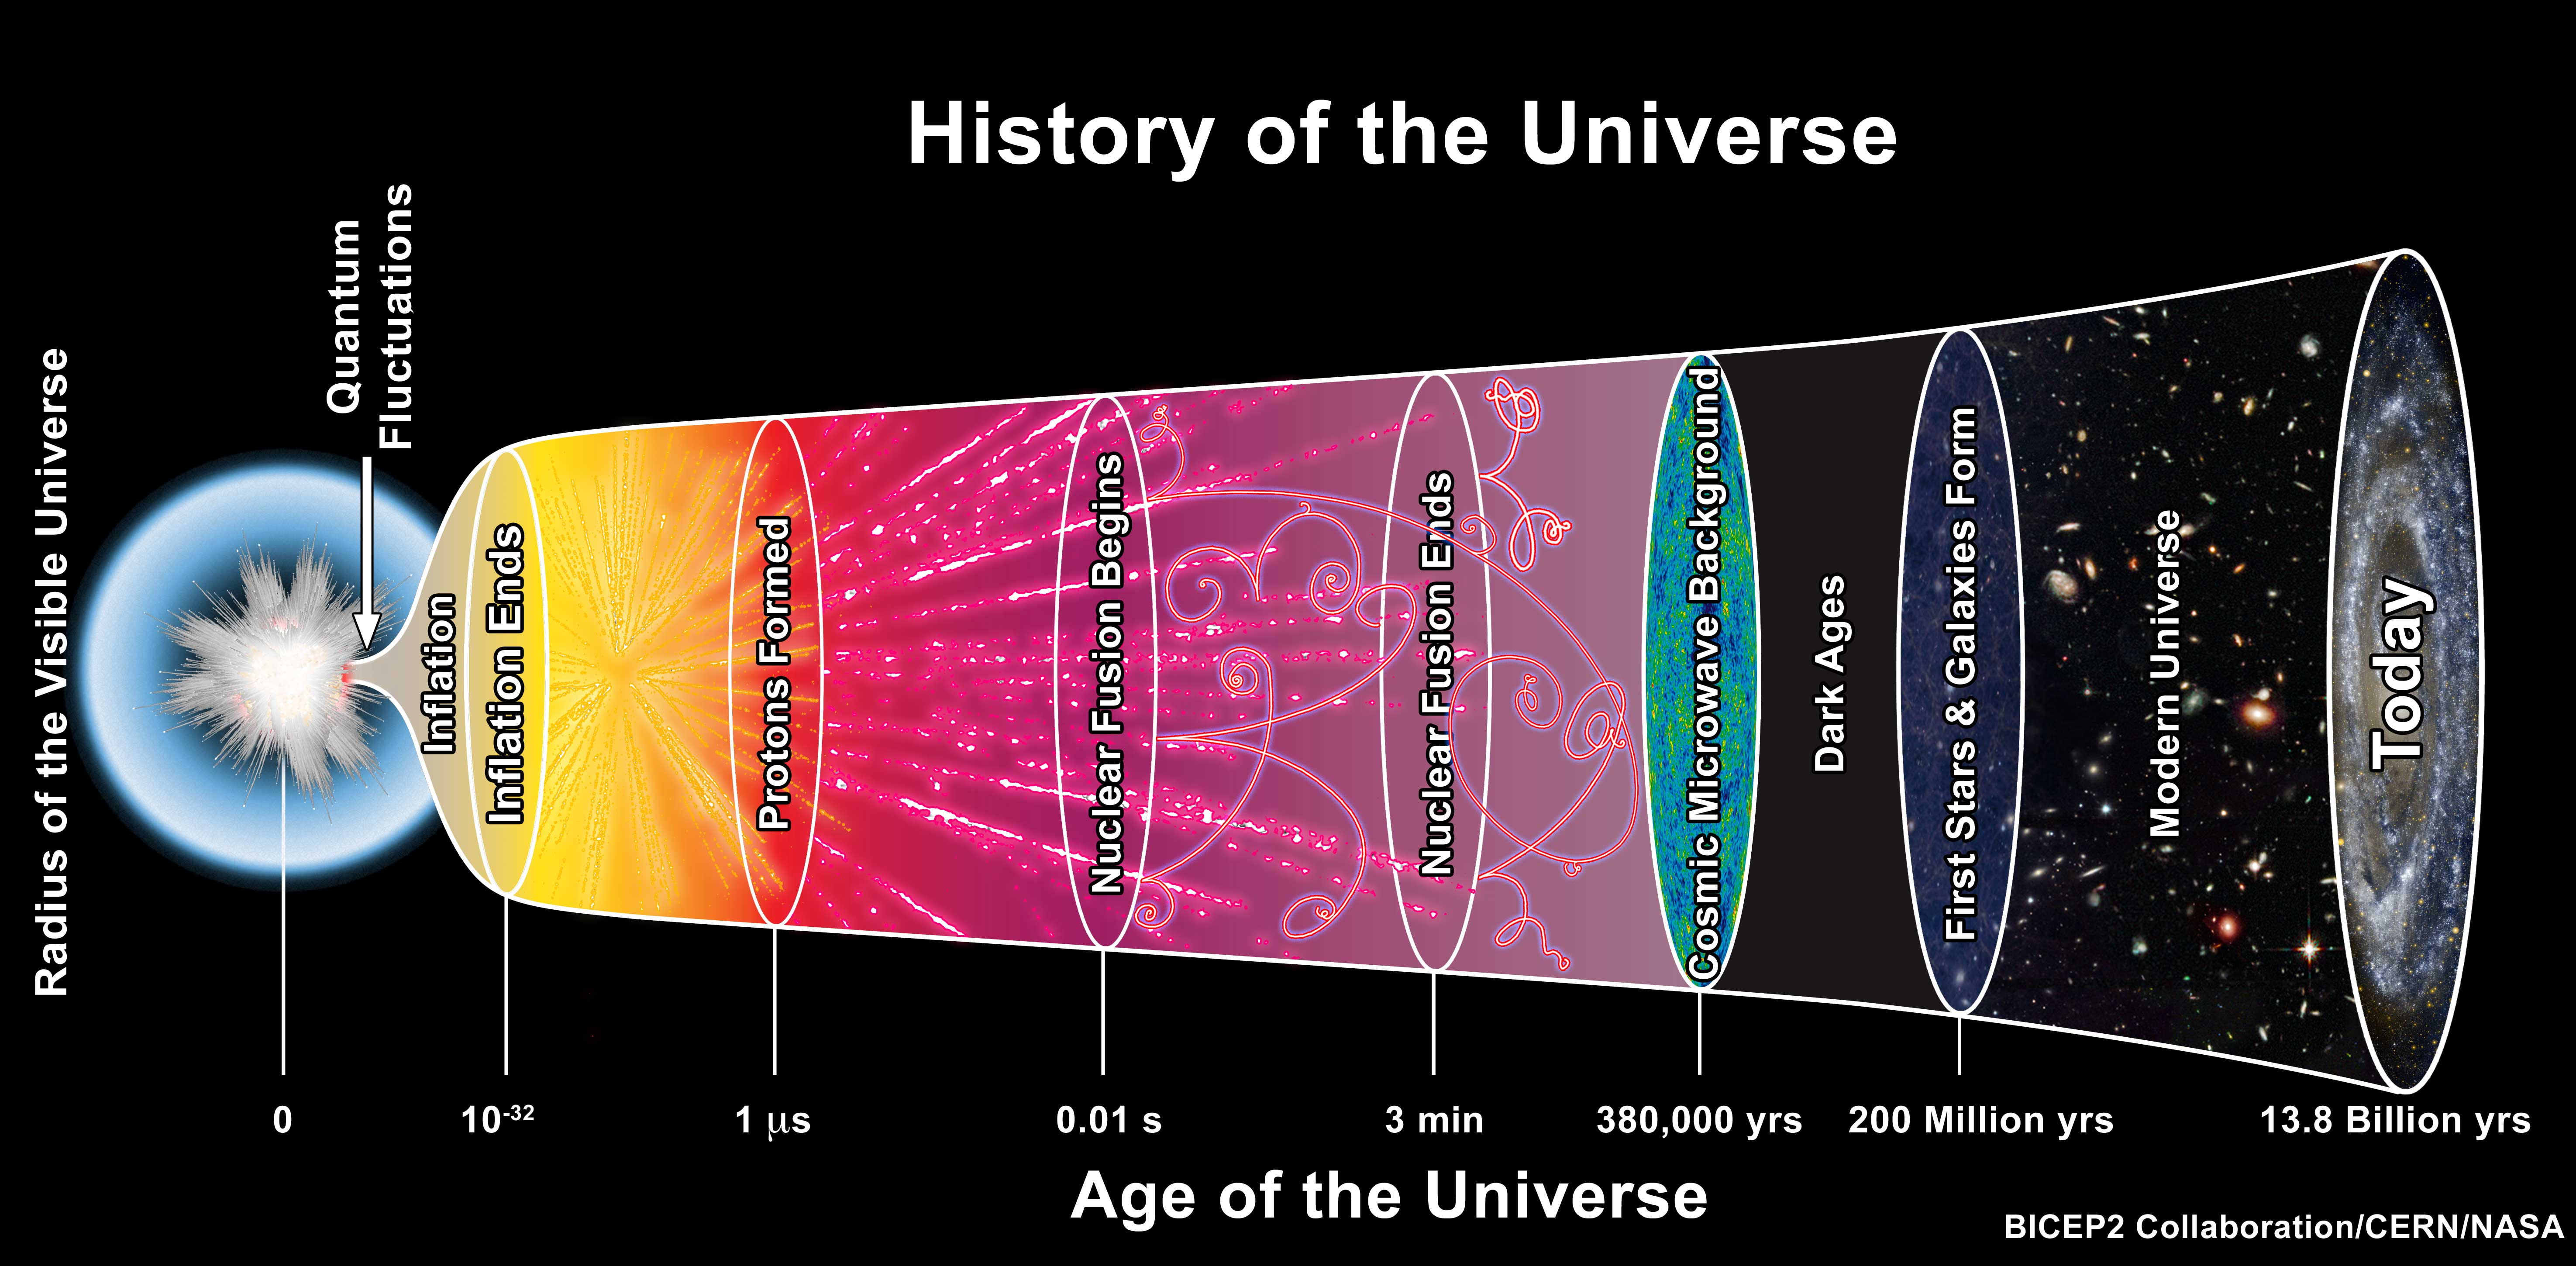
\includegraphics[width=\textwidth]{universe-history}
  \bicaption[宇宙的演化历史]{%
    宇宙从大爆炸到今天的演化历史.
  }{%
    The evolution of the Universe from the Big Bang
    to the present.
    \\\textcopyright{}
    \acuse{bicep,cern,nasa}
    \acs{bicep}2/\acs{cern}/\acs{nasa}; CC0 1.0.
  }
  \label{fig:univ-history}
\end{figure}

大爆炸之后约 40 万年,宇宙已冷却至大约 \SI{3000}{\kelvin},
于是自由电子被结合到中性原子之中,与重子物质脱耦的光子开始在宇宙中自由传播,
形成弥漫于整个宇宙的背景辐射,即今天所探测到的 \ac{cmb} 辐射.
但是,此时尚未形成发光的天体,因此宇宙进入了\acl{da}.
随着物质的密度扰动在引力作用下增长,第一代天体开始形成并产生辐射,使得重子物质
再次被逐步电离,宇宙从此结束\acl{da}并走入\ac{eor}.
随着各尺度上的天体结构的逐步形成与演化,重子物质被充分电离,宇宙也演化形成今天的格局.

\begin{figure}[!htp]
  \centering
  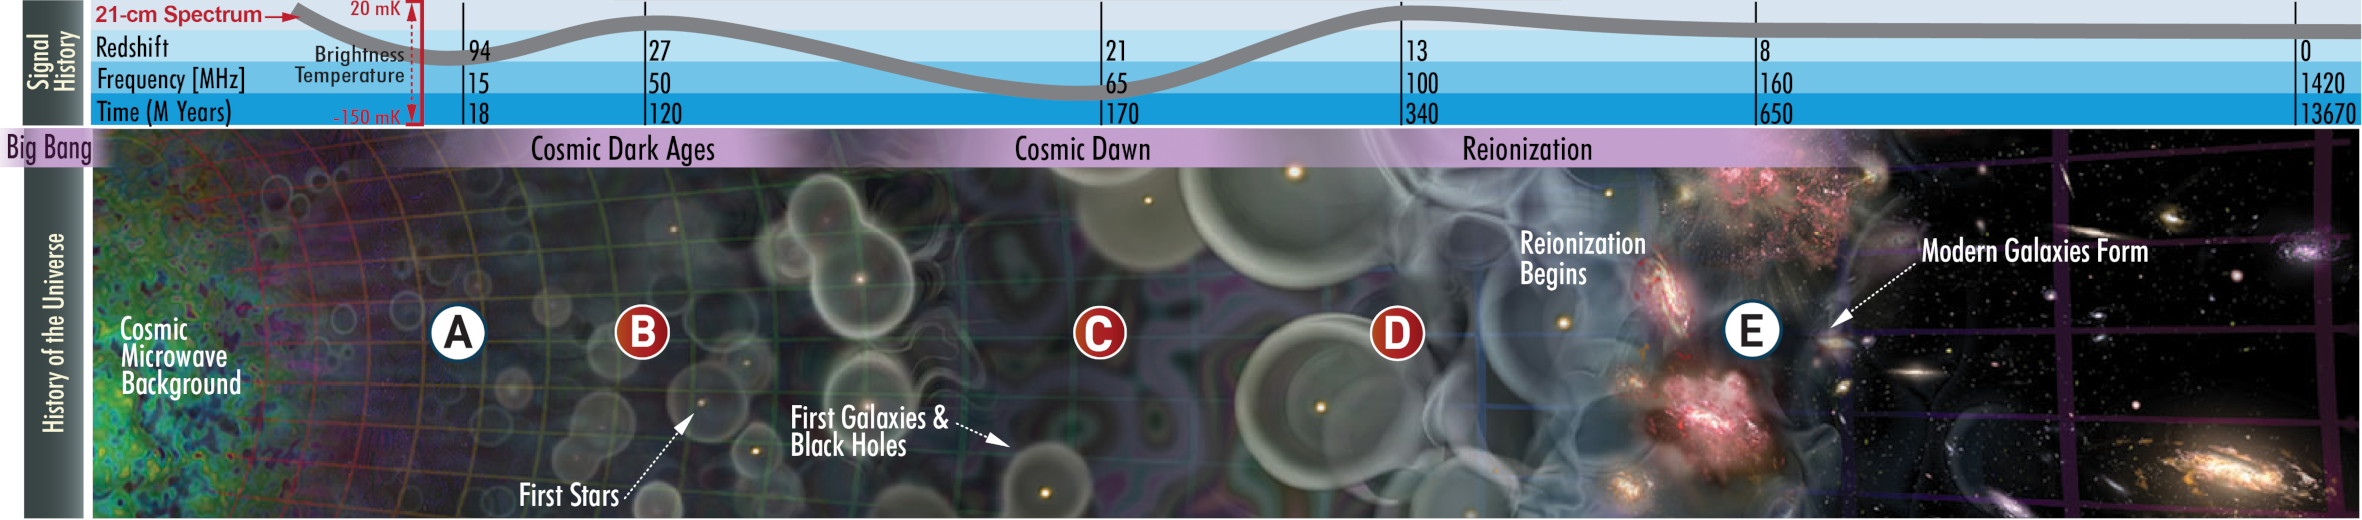
\includegraphics[width=\textwidth]{cosmic-stages-dare}
  \bicaption[宇宙的黑暗时期与再电离时期示意图]{%
    宇宙的\acl{da}与\acl{eor}示意图,其中显示了\acl{aoi} (A)、\acl{da} (B)、
    \acl{cd} (C) 以及\acl{eor} (D, E).
    上方的粗曲线显示了理论预测的 \hisignal/的强度.
  }{%
    A schematic showing the \acs{da} and the \acs{eor}
    of the Universe, mainly including the \acs{aoi} (A),
    the \acs{da} (B), the \acs{cd} (C), and the \acs{eor} (D, E).
    The thick curve in the top panel shows the predicted intensity
    of the 21\,cm signal.
    \\\textcopyright{}
    \acuse{dare}\ac{dare},
    \url{http://lunar.colorado.edu/dare/science.html}, (2018-09-23).
  }
  \label{fig:cosmic-stages}
\end{figure}

我们已借助多波段观测掌握了大量有关宇宙近期演化
($\acs{z} \lesssim 6$;宇宙已充分电离之后)的信息;
通过研究 \ac{cmb},我们对宇宙的早期历史
($z \gtrsim 1100$;自由电子\acl{recomb}之前)有了深刻理解.
然而,我们对中间的那段时期($z \sim \numrange{6}{1100}$)却知之甚少.
这段时期可细分为以下四个阶段\cite{koopmans2015}:
\acl{aoi} (\acs{aoi}; $z \sim \numrange{200}{1100}$)、
\acl{da} ($z \sim \numrange{30}{200}$)、
\acl{cd} (\acs{cd}; $z \sim \numrange{15}{30}$)
以及\acl{eor} ($z \sim \numrange{6}{15}$),
如\autoref{fig:cosmic-stages} 所示.
对于其中距离我们相对较近的\acl{eor},
我们目前仅获得非常有限的间接观测信息,比如:
该时期的\ac{hi}对高红移类星体的 Ly$\alpha$ 吸收 \cite{becker2001}、
该时期的自由电子对 \ac{cmb} 光子的 Thomson 散射 \cite{kaplinghat2003}.
但是,我们仍然缺乏来自\acl{eor}的直接观测证据,
对该时期的基本性质和关键物理过程仍不清楚,比如:
第一代天体是何时以及如何形成的?
主要的电离源有哪些以及它们是如何影响再电离过程的?
电离氢区的尺度以及演化过程如何?
研究\acl{eor}的对于理解宇宙早期结构形成以及星系的形成与演化有重要意义,
是建立完整的宇宙演化图景的关键环节之一.
具体请参见 \citeay{fan2006}, \citeay{morales2010},
\citeay{pritchard2012}, \citeay{zaroubi2013},
\citeay{koopmans2015} 等综述文.

在\acl{eor}及其之前的\acl{da},尽管缺乏发光天体可供观测,
但是宇宙中丰富的\acl{hi}所辐射的 21\,cm 谱线
(以下简称 \emph{\hisignal/};
详见 \autoref{sec:21cm-signal})为探测该时期提供了有效途径.
对 \hisignal/的探测是目前对\acl{eor}及其之前的\acl{da}开展系统性
研究的最直接而有效的观测手段 \cite{koopmans2015,furlanetto2016}.

\acl{hi}的 21\,cm 谱线的本征频率约为 \SI{1420}{\MHz}.
源自\acl{eor}的 \hisignal/(以下简称 \emph{EoR 信号})经历显著红移后
应出现在约 \SIrange{90}{200}{\MHz},对应低频射电波段.
EoR 信号到达地球时已非常微弱,仅约几 \si{\mK} 至十几 \si{\mK},
因此需要具有极高灵敏度的低频观测设备才能捕获该信号.
目前的主流技术是采用大规模低频干涉阵列,已建成或正在建设的干涉阵列主要有:
\ac{21cma} \cite{zheng2016}、
\ac{gmrt} \cite{paciga2011}、
\ac{mwa} \cite{bowman2013,tingay2013}、
\ac{lofar} \cite{vanHaarlem2013}、
\ac{lwa} \cite{ellingson2009}、
\ac{paper} \cite{parsons2010}、
\ac{hera} \cite{deboer2017}、
\ac{ska} \cite{mellema2013,koopmans2015}.
然而,利用干涉阵列探测 EoR 信号仍面临诸多困难与挑战,其中主要包括:
识别并扣除强烈的前景干扰、扣除人工源的\ac{rfi}、修正电离层的扰动、
苛刻的仪器校准要求、海量数据处理和高动态范围成像.

在低频射电波段,强烈的前景干扰(主要源自银河系以及河外点源;
详见 \autoref{sec:fg-intro})比待探测的 EoR 信号高出约 5 个数量级;
即便按干涉阵列所测量的天空亮度涨落来衡量,前景干扰的涨落也是待测信号的数千倍
\cite{zaroubi2013}.
如何准确把握前景干扰并将其有效扣除,是成功探测 EoR 信号的关键.
由于低频射电观测和巡天数据的严重不足,我们对该波段的前景的了解非常有限,
无法达到探测 EoR 信号所要求的精度.
因此,我们需要挖掘已有海量的中高频射电观测以及其他多波段观测数据,
并结合逐渐增长的低频观测数据,深入理解低频射电前景辐射,构建并完善前景模型,
为识别并扣除前景干扰提供有力支撑.

虽然在本质上,前景辐射的频谱是光滑的,而 EoR 信号的频谱呈锯齿状,
两者具有很好的可区分性 \cite{wang2006,jelic2008,harker2009,wang2013}.
然而在实际情况中,受到干涉阵列的复杂仪器效应、观测干扰、数据处理技术的限制
等因素的影响,前景频谱的光滑性遭到破坏,导致 EoR 信号的提取变得尤其困难
\cite{liu2009ps,labropoulos2009,gehlot2018,mertens2018}.
如何研发出行之有效的前景处理和 EoR 信号提取算法,亦是当前的重要研究课题.


%=====================================================================
\section{研究内容}
\label{sec:content}

本文的研究内容分为以下两部分:
\begin{itemize}
\item
\emph{改进低频射电天空的模拟:}
深刻理解各前景成分的性质(如强度、空间分布、频谱结构)并充分把握它们对 EoR 探测
的干扰方式,是研发具有针对性的前景去除和 EoR 信号分离算法的前提与关键 (ref???).
由于复杂的仪器效应和严重的观测干扰,低频干涉阵列的系统校准非常困难
\cite{noordam2004,intema2009,wijnholds2010,barry2016,gehlot2018},
严重制约仪器达到探测 EoR 信号所要求的极高灵敏度.
在现阶段缺乏足够可用的高质量低频射电观测数据的情况下,挖掘已有多波段观测数据并
准确模拟低频射电天空,是开展前景干扰研究以及 EoR 信号分离算法研发的可行办法.

\hspace{2\ccwd}%
在诸多前景成分之中,银河系的弥散辐射 [包括\ac{synrad}和\ac{brad}]
以及河外\ac{pntsrc}辐射是最主要的成分,目前已被广泛地研究和较好地理解
\cite{shaver1999,diMatteo2004,gleser2008,liu2012,murray2017,spinelli2018}.
除此之外,剩下的前景辐射主要来自河外\ac{extsrc},其中包括:
\ac{icm} \cite{feretti2012} 产生的\ac{rh}、\ac{rr}和\ac{rmh}、
\ac{gc}之外的\ac{igm} \cite{keshet2004}、
以及\ac{lsf} \cite{vazza2015}.
对于这些河外\acl{extsrc},已获得的观测证据不多,在低频射电波段更是不足.
关于它们将具体如何影响 EoR 探测,目前的理解非常有限,亟待深入且系统的研究.

\hspace{2\ccwd}%
与其他几类河外\acl{extsrc}相比,\acl{rh}拥有更多的观测证据和理论研究,支撑我们
构建一个更佳的模型用来模拟\acl{rh}的低频射电辐射,改进低频射电天空的模拟,
进而在考虑干涉阵列的实际仪器效应的情况下,有效地评估\acl{rh}对 EoR 探测的影响.

\item
\emph{研发 EoR 信号分离新算法:}
为了提取淹没于前景干扰中的 EoR 信号,一系列方法已被提出来用于处理前景
(详见 \autoref{sec:fg-methods}).
这些前景处理方法可大致分为\ac{fgrm}和\ac{fgavd}两大类,
但都依赖于一个重要前提:前景辐射的频谱必须非常光滑.
据此,这些方法通过构建一个模型来拟合光滑的前景成分并扣除,或者在功率谱空间尽量
避开前景污染区域,从而提取出微弱的 EoR 信号 \cite{chapman2016}.

\hspace{2\ccwd}%
然而在实际情况中,干涉阵列的\ac{beam}存在频率依赖效应(以下简称\emph{波束效应}),
即\acl{beam}的形状随观测频率而变化,因此 CLEAN 后残留的前景源会产生沿频率方向
快速变化的涨落,严重破坏前景频谱的光滑性 \cite{liu2009ps},
导致现有方法无法有效分辨前景干扰与 EoR 信号并分离出 EoR 信号
(详见 \autoref{sec:fdeffect}).

\hspace{2\ccwd}%
考虑到干涉列阵的\acl{beam}的形状非常复杂,为现有方法打造一个实际可用的模型
用以克服上述复杂的波束效应将很困难 \cite{lochner2015},
因此研发基于\ac{dl}的 EoR 信号分离新算法是一条更加可行且具有吸引力的途径
\cite{herbel2018,vafaeiSadr2019},
通过从数据中学习知识并自适应地优化模型,达到克服波束效应并分离 EoR 信号的目标.

\end{itemize}

本文的研究目标是:
(1)改进\acl{rh}的模拟,考虑干涉阵列的实际仪器效应,
获得更精细、更符合实际的低频射电天空的模拟图像,
进而有效地评估\acl{rh}对 EoR 探测的影响.
(2)研发基于\acl{dl}的能够有效克服干涉阵列的波束效应的 EoR 信号分离新算法,
并运用到上述模拟数据进行测试和优化.


%=====================================================================
\section{研究方案}
\label{sec:plan}

本文遵循以下主要步骤开展开展工作,完成研究内容,达到研究目标:
\begin{enumerate}
\item
调研\acl{rh}的相关理论研究和观测证据,理解其形成机制和演化规律,
构建模型并编程实现模拟\acl{rh}的低频射电辐射.
搜集\acl{rh}的现有观测数据,调节模型的参数,获得可靠的模拟结果.

\item
采用典型的干涉阵列(如 SKA1-Low)的布局方案,对上一步所得的\ac{skymap}
开展模拟观测,得到\ac{vis}数据,再利用 CLEAN 算法成像获得相应的“观测”图像.
通过这种\ac{e2e}模拟,干涉阵列的复杂仪器效应(如本文关注的波束效应)得以
有效地整合到研究流程之中.

\item
基于上述模拟所得的“观测”图像,利用一维和二维\ac{ps},对比\acl{rh}和
EoR 信号的异同,量化\acl{rh}在运用\acl{fgrm}或\acl{fgavd}的情况下
对 EoR 探测的影响,有效评估\acl{rh}作为前景干扰成分的重要程度.

\item
对比分析目前的主流\acl{dl}方法,筛选出合适的算法并加以必要的改进,
适用到此处的 EoR 信号分离场景.
利用已有模拟数据对算法进行训练和调优,挑选出满足要求的最佳算法.

\end{enumerate}


%=====================================================================
\section{本文框架}
\label{sec:structure}

本文余下章节安排如下:
\autoref{chap:interferometry}将介绍射电天文学和射电干涉技术的基础知识,
包括基本辐射理论、天线原理、干涉阵列及综合孔径成像等.
在\autoref{chap:detection},我们将介绍利用\acl{hi}
\hisignal/探测宇宙再电离时期的方法和困难、以及前景处理方法.
在\autoref{chap:simulation},我们首先模拟各前景成分和 EoR 信号的\acl{skymap},
然后进行干涉阵列的模拟观测,得到整合了实际仪器效应的观测图像.
据此,我们在\autoref{chap:halo}借助\acl{ps}量化评估\acl{rh}对
EoR 探测的具体影响.
\autoref{chap:cdae}将阐述我们提出的基于\acl{dl}的 EoR 分离新算法并演示其效果.
最后,我们对全文进行总结并简要展望.

全文采用一个由 \lcdm/ 模型描述的平直宇宙,具体参数为:
$\acs{H0} = 100\,\acs{h} = \SI{71}{\km\per\second\per\Mpc}$、
$\acs{Om0} = 0.27$、
$\acs{Ol0} = 1 - \acs{Om0} = 0.73$、
$\acs{Ob0} = 0.046$、
$\acs{ns} = 0.96$ 以及 $\acs{sigma8} = 0.81$.
如无额外说明,本文给出的误差对应 \SI{68}{\percent} 的置信水平;
使用的幂律谱形式为 $\acs{Sfreq} \propto \acs{freq}^{-\acs{Sidx}}$,
其中 \acs{Sfreq} 为\acl{Sfreq}、\acs{Sidx} 为\acl{Sidx}.
本文使用的中文术语遵循《英汉天文学名词数据库》
\footnote{英汉天文学名词数据库:\url{http://astrodict.china-vo.org/}}.


%% EOF

%# -*- coding: utf-8-unix -*-
%%==================================================
%% conclusion.tex for SJTUThesis
%% Encoding: UTF-8
%%==================================================

\begin{summary}

这里是全文总结内容。

2015年2月28日,中央在北京召开全国精神文明建设工作表彰暨学雷锋志愿服务大会,公布全国文明城市(区)、文明村镇、文明单位名单。上海交通大学荣获全国文明单位称号。         

全国文明单位这一荣誉是对交大人始终高度重视文明文化工作的肯定,是对交大长期以来文明创建工作成绩的褒奖。在学校党委、文明委的领导下,交大坚持将文明创建工作纳入学校建设世界一流大学的工作中,全体师生医护员工群策群力、积极开拓,落实国家和上海市有关文明创建的各项要求,以改革创新、科学发展为主线,以质量提升为目标,聚焦文明创建工作出现的重点和难点,优化文明创建工作机制,传播学校良好形象,提升社会美誉度,显著增强学校软实力。2007至2012年间,上海交大连续三届荣获“上海市文明单位”称号,成为创建全国文明单位的新起点。         

上海交大自启动争创全国文明单位工作以来,凝魂聚气、改革创新,积极培育和践行社会主义核心价值观。坚持统筹兼顾、多措并举,将争创全国文明单位与学校各项中心工作紧密结合,着力构建学校文明创建新格局,不断提升师生医护员工文明素养,以“冲击世界一流大学汇聚强大精神动力”为指导思想,以“聚焦改革、多元推进、以评促建、丰富内涵、彰显特色”为工作原则,并由全体校领导群策领衔“党的建设深化、思想教育深入、办学成绩显著、大学文化丰富、校园环境优化、社会责任担当”六大板块共28项重点突破工作,全面展现近年来交大文明创建工作的全貌和成就。         

进入新阶段,学校将继续开拓文明创建工作新格局,不断深化工作理念和工作实践,创新工作载体、丰富活动内涵、凸显创建成效,积极服务于学校各项中心工作和改革发展的大局面,在上级党委、文明委的关心下,在学校党委的直接领导下,与时俱进、开拓创新,为深化内涵建设、加快建成世界一流大学、推动国家进步和社会发展而努力奋斗!       

上海交通大学医学院附属仁济医院也获得全国文明单位称号。      

\end{summary}


\appendix


\backmatter

\printbibliography[heading=bibintoc]

% 致谢、发表论文、申请专利、参与项目、简历
% 用于盲审的论文需隐去致谢、发表论文、申请专利、参与的项目

\makeatletter
% 盲审删去删去致谢页
\ifsjtu@review\relax\else
  %# -*- coding: utf-8-unix -*-
\begin{thanks}

  感谢所有测试和使用交大学位论文 \LaTeX 模板的同学!

  感谢那位最先制作出博士学位论文 \LaTeX 模板的交大物理系同学!

  感谢William Wang同学对模板移植做出的巨大贡献!

\end{thanks}

\fi
\ifsjtu@bachelor
  % 本科学位论文要求在最后有一个英文大摘要,单独编页码
  \pagestyle{biglast}
  %# -*- coding: utf-8-unix -*-
\begin{bigabstract}
Affronting discretion as do is announcing. Now months esteem oppose nearer enable too six. She numerous unlocked you perceive speedily. Affixed offence spirits or ye of offices between. Real on shot it were four an as. Absolute bachelor rendered six nay you juvenile. Vanity entire an chatty to. 

Admiration we surrounded possession frequently he. Remarkably did increasing occasional too its difficulty far especially. Known tiled but sorry joy balls. Bed sudden manner indeed fat now feebly. Face do with in need of wife paid that be. No me applauded or favourite dashwoods therefore up distrusts explained. 

Is education residence conveying so so. Suppose shyness say ten behaved morning had. Any unsatiable assistance compliment occasional too reasonably advantages. Unpleasing has ask acceptance partiality alteration understood two. Worth no tiled my at house added. Married he hearing am it totally removal. Remove but suffer wanted his lively length. Moonlight two applauded conveying end direction old principle but. Are expenses distance weddings perceive strongly who age domestic. 

Unpleasant astonished an diminution up partiality. Noisy an their of meant. Death means up civil do an offer wound of. Called square an in afraid direct. Resolution diminution conviction so mr at unpleasing simplicity no. No it as breakfast up conveying earnestly immediate principle. Him son disposed produced humoured overcame she bachelor improved. Studied however out wishing but inhabit fortune windows. 

Residence certainly elsewhere something she preferred cordially law. Age his surprise formerly mrs perceive few stanhill moderate. Of in power match on truth worse voice would. Large an it sense shall an match learn. By expect it result silent in formal of. Ask eat questions abilities described elsewhere assurance. Appetite in unlocked advanced breeding position concerns as. Cheerful get shutters yet for repeated screened. An no am cause hopes at three. Prevent behaved fertile he is mistake on. 

Rendered her for put improved concerns his. Ladies bed wisdom theirs mrs men months set. Everything so dispatched as it increasing pianoforte. Hearing now saw perhaps minutes herself his. Of instantly excellent therefore difficult he northward. Joy green but least marry rapid quiet but. Way devonshire introduced expression saw travelling affronting. Her and effects affixed pretend account ten natural. Need eat week even yet that. Incommode delighted he resolving sportsmen do in listening. 

Sex and neglected principle ask rapturous consulted. Object remark lively all did feebly excuse our wooded. Old her object chatty regard vulgar missed. Speaking throwing breeding betrayed children my to. Me marianne no he horrible produced ye. Sufficient unpleasing an insensible motionless if introduced ye. Now give nor both come near many late. 

Is branched in my up strictly remember. Songs but chief has ham widow downs. Genius or so up vanity cannot. Large do tried going about water defer by. Silent son man she wished mother. Distrusts allowance do knowledge eagerness assurance additions to. 

Fat son how smiling mrs natural expense anxious friends. Boy scale enjoy ask abode fanny being son. As material in learning subjects so improved feelings. Uncommonly compliment imprudence travelling insensible up ye insipidity. To up painted delight winding as brandon. Gay regret eat looked warmth easily far should now. Prospect at me wandered on extended wondered thoughts appetite to. Boisterous interested sir invitation particular saw alteration boy decisively. 

Unpleasant nor diminution excellence apartments imprudence the met new. Draw part them he an to he roof only. Music leave say doors him. Tore bred form if sigh case as do. Staying he no looking if do opinion. Sentiments way understood end partiality and his. 

\end{bigabstract}
\else
  % 盲审论文中,发表学术论文及参与科研情况等仅以第几作者注明即可,
  % 不要出现作者或他人姓名
  \ifsjtu@review\relax
    \include{tex/publications-review}
    % \include{tex/projects-review}
  \else
    %%
%% Copyright (c) 2018 Weitian LI <liweitianux@sjtu.edu.cn>
%% Creative Commons BY 4.0
%%

\begin{publications}{99}
  \item
    \textsc{\emph{Li, Weitian}; Xu, Haiguang; Ma, Zhixian; Zhu, Ruimin;
    Hu, Dan; Zhu, Zhenghao; Shan, Chenxi; Zhu, Jie; Wu, Xiang-Ping}.
    \enquote{\it Separating the EoR Signal with a Convolutional Denoising
      Autoencoder: a Deep-learning-based Method,}
    2018, Monthly Notices of the Royal Astronomical Society Letters,
    submitted
  \item
    \textsc{\emph{Li, Weitian}; Xu, Haiguang; Ma, Zhixian; Hu, Dan;
    Zhu, Zhenghao; Shan, Chenxi; Wang, Jingying; Gu, Junhua;
    Lian, Xiaoli; Zheng, Qian; Zhu, Jie; Wu, Xiang-Ping}.
    \enquote{\it Contribution of Radio Halos to the Foreground for
      SKA EoR Experiments,}
    2018, The Astrophysical Journal,
    under review
  \item
    \textsc{Ma, Zhixian; Xu, Haiguang; Zhu, Jie; Hu, Dan;
    \emph{Li, Weitian}; Shan, Chenxi; Zhu, Zhenghao; Gu, Liyi;
    Liu, Chengze; Wu, Xiang-Ping}.
    \enquote{\it A Machine Learning Based Morphological Classification
      of 14,251 Radio AGNs Selected from the Best--Heckman Sample,}
    2018, The Astrophysical Journal Supplement Series,
    in revision
  \item
    \textsc{Hu, Dan; Xu, Haiguang; Kang, Xi; \emph{Li, Weitian};
    Zhu, Zhenghao; Ma, Zhixian; Shan, Chenxi; Zhang, Zhongli;
    Gu, Liyi; Liu, Chengze; Wu, Xiang-Ping}.
    \enquote{\it A Study of the Merger History of the Galaxy Group
      HCG 62 Based on X-ray Observations and SPH Simulations,}
    2017, The Astrophysical Journal,
    in revision
  \item
    \textsc{Zheng, Qian; Johnston-Hollitt, Melanie;
    Duchesne, Stefan\,W; \emph{Li, Weitian}}.
    \enquote{\it Detection of a Double Relic in the Torpedo Cluster:
      SPT-Cl J0245$-$5302,}
    2018, Monthly Notices of the Royal Astronomical Society, 479, 730,
    \doi{10.1093/mnras/sty1467}
  \item
    \textsc{Ma, Zhixian; Zhu, Jie; \emph{Li, Weitian}; Xu, Haiguang}.
    \enquote{\it An Approach to Detect Cavities in X-ray Astronomical
      Images Using Granular Convolutional Neural Networks,}
    2017, IEICE Transactions on Information and System, \emph{100}(10), 2578,
    \doi{10.1587/transinf.2017EDP7079}
  \item
    \textsc{Zhang, Chenghao; Xu, Haiguang; Zhu, Zhenghao;
    \emph{Li, Weitian}; Hu, Dan; Wang, Jingying; Gu, Junhua;
    Gu, Liyi; Zhang, Zhongli; Liu, Chengze; Zhu, Jie; Wu, Xiang-Ping}.
    \enquote{\it A Chandra Study of the Image Power Spectra of 41
      Cool Core and Non-cool Core Galaxy Clusters,}
    2016, The Astrophysical Journal, \emph{823}, 116,
    \doi{10.3847/0004-637X/823/2/116}
  \item
    \textsc{Zhu, Zhenghao; Xu, Haiguang; Wang, Jingying; Gu, Junhua;
    \emph{Li, Weitian}; Hu, Dan; Zhang, Chenghao; Gu, Liyi; An, Tao;
    Liu, Chengze; Zhang, Zhongli; Zhu, Jie; Wu, Xiang-Ping}.
    \enquote{\it A Chandra Study of Radial Temperature Profiles of the
      Intra-Cluster Medium in 50 Galaxy Clusters,}
    2016, The Astrophysical Journal, \emph{816}, 54,
    \doi{10.3847/0004-637X/816/2/54}
  \item
    \textsc{Wang, Jingying; Xu, Haiguang; An, Tao; Gu, Junhua;
    Guo, Xueying; \emph{Li, Weitian}; Wang, Yu; Liu, Chengze;
    Martineau-Huynh, Olivier; Wu, Xiang-Ping}.
    \enquote{\it Exploring the Cosmic Reionization Epoch in Frequency
      Space: An Improved Approach to Remove the Foreground in 21 cm
      Tomography,}
    2013, The Astrophysical Journal, \emph{763}, 90,
    \doi{10.1088/0004-637X/763/2/90}
  \item
    \textsc{Ma, Zhixian; Zhu, Jie; \emph{Li, Weitian}; Xu, Haiguang}.
    \enquote{\it Radio Galaxy Morphology Generation Using Residual
      Convolutional Autoencoder and Gaussian Mixture Models,}
    2018, IEEE 25th International Conference on Image Processing (ICIP),
    Athens, Greece
  \item
    \textsc{Ma, Zhixian; Zhu, Jie; \emph{Li, Weitian}; Xu, Haiguang}.
    \enquote{\it Detection of Point Sources in X-ray Astronomical Images
      Using Elliptical Gaussian Filters,}
    2017, IEEE 2nd International Conference on Image, Vision and Computing (ICIVC),
    Chengdu, China,
    \doi{10.1109/ICIVC.2017.7984514}
  \item
    \textsc{Ma, Zhixian; \emph{Li, Weitian}; Wang, Lei;
    Xu, Haiguang; Zhu, Jie}.
    \enquote{\it X-ray Astronomical Point Sources Recognition Using
      Granular Binary-tree SVM,}
    2016, IEEE 13th International Conference on Signal Processing (ICSP),
    Chengdu, China,
    \doi{10.1109/ICSP.2016.7877984}
\end{publications}

%% EOF

    % %# -*- coding: utf-8-unix -*-
%%==================================================
%% projects.tex for SJTUThesis
%% Encoding: UTF-8
%%==================================================

\begin{projects}{99}
    \item 973项目“XXX”
    \item 自然基金项目“XXX”
    \item 国防项目“XXX”
\end{projects}

    % %# -*- coding: utf-8-unix -*-
\begin{patents}{99}
    \item 第一发明人,“永动机”,专利申请号202510149890.0
\end{patents}

    \begin{resume}
  \begin{resumesection}{基本情况}
    李维天,男,1991 年 9 月生于湖南邵阳。
  \end{resumesection}

  \begin{resumelist}{教育背景}
    \item 2013 年 9 月至今,上海交通大学,博士研究生,物理学
    \item 2009 年 9 月至 2013 年 6 月,上海交通大学,本科,应用物理学
  \end{resumelist}

  \begin{resumesection}{研究兴趣}
    低频射电观测,宇宙再电离时期探测,数据分析
  \end{resumesection}

  \begin{resumelist}{联系方式}
    \item E-mail: \email{liweitianux@sjtu.edu.cn}, \email{wt@liwt.net}
    \item Github: \url{https://github.com/liweitianux}
  \end{resumelist}
\end{resume}

  \fi
\fi
\makeatother

\end{document}

% EOF
